\section{\sys{}: A Reference Defense}\label{sec:design}

\sys{} (Agent Step-Up) is the design we use as a control in every experiment. It is deliberately conventional:
it combines the digest-bound approval of SUDP and ADR~0030 with a second device, typed card rendering and
argument-complete grants. It exists so that each attack and each measurement has a defense whose properties are
proven rather than assumed. It reuses no code from aiAuthZ, but it follows the same principle: the decision
lives in a trust domain the agent cannot reach.

\subsection{Protocol}

\Cref{fig:protocol} shows a challenged call. The agent holds only a session token. It sends a tool call, with an
optional free-text explanation, to the gateway. The gateway canonicalizes the call into a descriptor $\Desc$,
computes $\dig=\Hash(\JCS(\Desc))$, and asks its policy for \code{allow}, \code{deny} or \code{challenge}. On a
challenge it stores the pending approval and returns \code{202} with an opaque approval identifier; the agent
receives no code, no card text and no challenge. The user opens the approval page, which the gateway serves to
the user's own phone and never relays through the agent. The page shows a card rendered from $\Desc$ and asks the
platform authenticator for an assertion over the challenge
\[
c \;=\; \Hash\!\big(\JCS(\{\texttt{tag}{:}\,\texttt{"ASU-APPROVAL-v2"},\ \texttt{digest}{:}\,\dig,\
\texttt{approval\_id}{:}\,\mathit{id},\ \texttt{nonce}{:}\,n,\ \texttt{grant\_digest}{:}\,g\})\big),
\]
where $g$ is the digest of a delegated grant if the user ticks ``allow similar'' and \code{null} otherwise.
Encoding the challenge as a canonical JSON object rather than a concatenation makes it injective in its fields,
which closes \AB{8}. The gateway verifies the assertion against $pk_U$, the expected origin and relying party,
with user verification required, and stores it as a receipt. When the agent retries with the identifier, the
gateway atomically moves the approval from approved to consumed and executes the \emph{stored} descriptor. If the
agent resubmits arguments and their digest differs, the gateway answers \code{409 effect\_mismatch} and nothing
runs (\AB{10}). A token mode replaces direct execution with a short-lived Ed25519 token over
$\{\dig,\mathit{aud},\mathit{exp},\mathit{jti}\}$ that the resource verifies, including single use of
$\mathit{jti}$. Every step is appended to a hash-chained audit log, keyed with an HMAC so that a party without the
key cannot rewrite it, and receipts can be verified offline from $pk_U$ and the relying party identifier alone.

\begin{figure}[t]
\centering
\resizebox{\textwidth}{!}{% Figure: message sequence of a challenged call in ASU
\begin{tikzpicture}[x=1cm,y=1cm,font=\scriptsize,>={Stealth[length=4pt]},
  actor/.style={draw=inkgray,rounded corners=2pt,minimum width=22mm,minimum height=6.5mm,fill=white,font=\footnotesize\bfseries},
  msg/.style={->,thick,inkgray},
  note/.style={font=\scriptsize,align=left,anchor=north west,text width=40mm,inner sep=1pt},
  lab/.style={font=\scriptsize,above=1pt,inner sep=1pt,fill=white}]
  % lanes: agent 0, gateway 5, phone 10, resource 14.6
  \def\xa{0}\def\xg{5}\def\xd{10}\def\xr{14.6}
  \def\yend{-11.4}
  \begin{scope}[on background layer]
    \fill[untrustred] (-1.3,0.5) rectangle (1.3,\yend);
    \fill[trustgreen] (3.7,0.5) rectangle (11.3,\yend);
  \end{scope}
  \foreach \x/\n/\t in {\xa/A/{Agent}, \xg/G/{Gateway}, \xd/D/{User's phone}, \xr/R/{Resource}}{
    \node[actor] (\n) at (\x,0) {\t};
    \draw[gray!70,dashed] (\x,-0.35) -- (\x,\yend);
  }
  \node[font=\scriptsize,text=narrorange!80!black,anchor=north] at (\xa,\yend-0.05) {agent's reach};
  \node[font=\scriptsize,text=noexaqua!60!black,anchor=north] at (7.5,\yend-0.05) {trusted, unreachable by the agent};

  % 1 call
  \draw[msg] (\xa,-1.0) -- node[lab] {tool call $q$, explanation $e$} (\xg,-1.0);
  \node[note] at (\xg+0.15,-1.15) {$\Desc=\mathsf{Canon}(q)$, $\dig=\Hash(\JCS(\Desc))$;\\ policy returns \code{challenge}};
  % 2 202
  \draw[msg] (\xg,-2.4) -- node[lab] {\code{202} and approval id only} (\xa,-2.4);
  % 3 open page
  \draw[msg] (\xd,-3.3) -- node[lab] {open page (TLS, signed-in user)} (\xg,-3.3);
  % 4 card + challenge
  \draw[msg] (\xg,-4.2) -- node[lab] {card $\mathsf{Render}(\Desc)$, grant offer, challenge $c$} (\xd,-4.2);
  \node[note,text width=30mm] at (\xd+0.15,-4.35) {user reads the card;\\ passkey signs $c$ with user verification};
  % 5 assertion
  \draw[msg] (\xd,-5.6) -- node[lab] {assertion over $c$ (covers $g$ if ticked)} (\xg,-5.6);
  \node[note] at (\xg+0.15,-5.75) {verify with $pk_U$, origin and relying party;\\ store the receipt};
  % 6 retry
  \draw[msg] (\xa,-7.0) -- node[lab] {retry with id [and args$'$]} (\xg,-7.0);
  \node[note] at (\xg+0.15,-7.15) {$\dig'\neq\dig \Rightarrow$ \code{409};\\ otherwise approved $\to$ consumed};
  % 7 execute
  \draw[msg] (\xg,-8.6) -- node[lab,pos=0.62] {execute stored $\Desc$, or token $\{\dig,\mathit{aud},\mathit{exp},\mathit{jti}\}$} (\xr,-8.6);
  % 8 result
  \draw[msg] (\xg,-9.6) -- node[lab] {result and receipt id} (\xa,-9.6);
  \node[note] at (\xg+0.15,-9.75) {append to the keyed hash chain};
\end{tikzpicture}
\unskip}
\caption{A challenged tool call in \sys{}. The agent sees only the approval identifier and the outcome. The card,
the challenge and the assertion travel between the gateway and the user's phone, and the gateway executes the
stored descriptor rather than the agent's resubmitted arguments.}
\label{fig:protocol}
\end{figure}

\subsection{What the card shows and why}\label{sec:card}

Several attacks in \cref{sec:attacks} target the card itself, so the card follows six rules. (i) Values are typed and quoted, so a boolean and a string never render alike, and a property
test checks that distinct digests render distinct cards (\AB{6}). (ii) Characters outside a printable allow-list
are escaped and flagged, runs of blank glyphs collapse to a counted marker, and long values are capped with an
explicit expand control and a risk line (\AB{4}). (iii) Argument names chosen by the agent appear only in a
separate ``Arguments'' section with a fixed \code{arg.} prefix, never as trusted labels (\AB{5}). (iv) Every
recipient, account, URL and path argument is a target, the title lists all of them, and a first-time-recipient
check applies to each one (\AB{2}). (v) Any interpreter invoked with inline code, such as \code{bash -c} or
\code{python -c}, is flagged. (vi) The agent's explanation is collapsed by default and labeled untrusted.
\Cref{fig:cards} shows three cards as the phone renders them.

\begin{figure}[t]
\centering
\begin{subfigure}[t]{0.32\textwidth}\centering
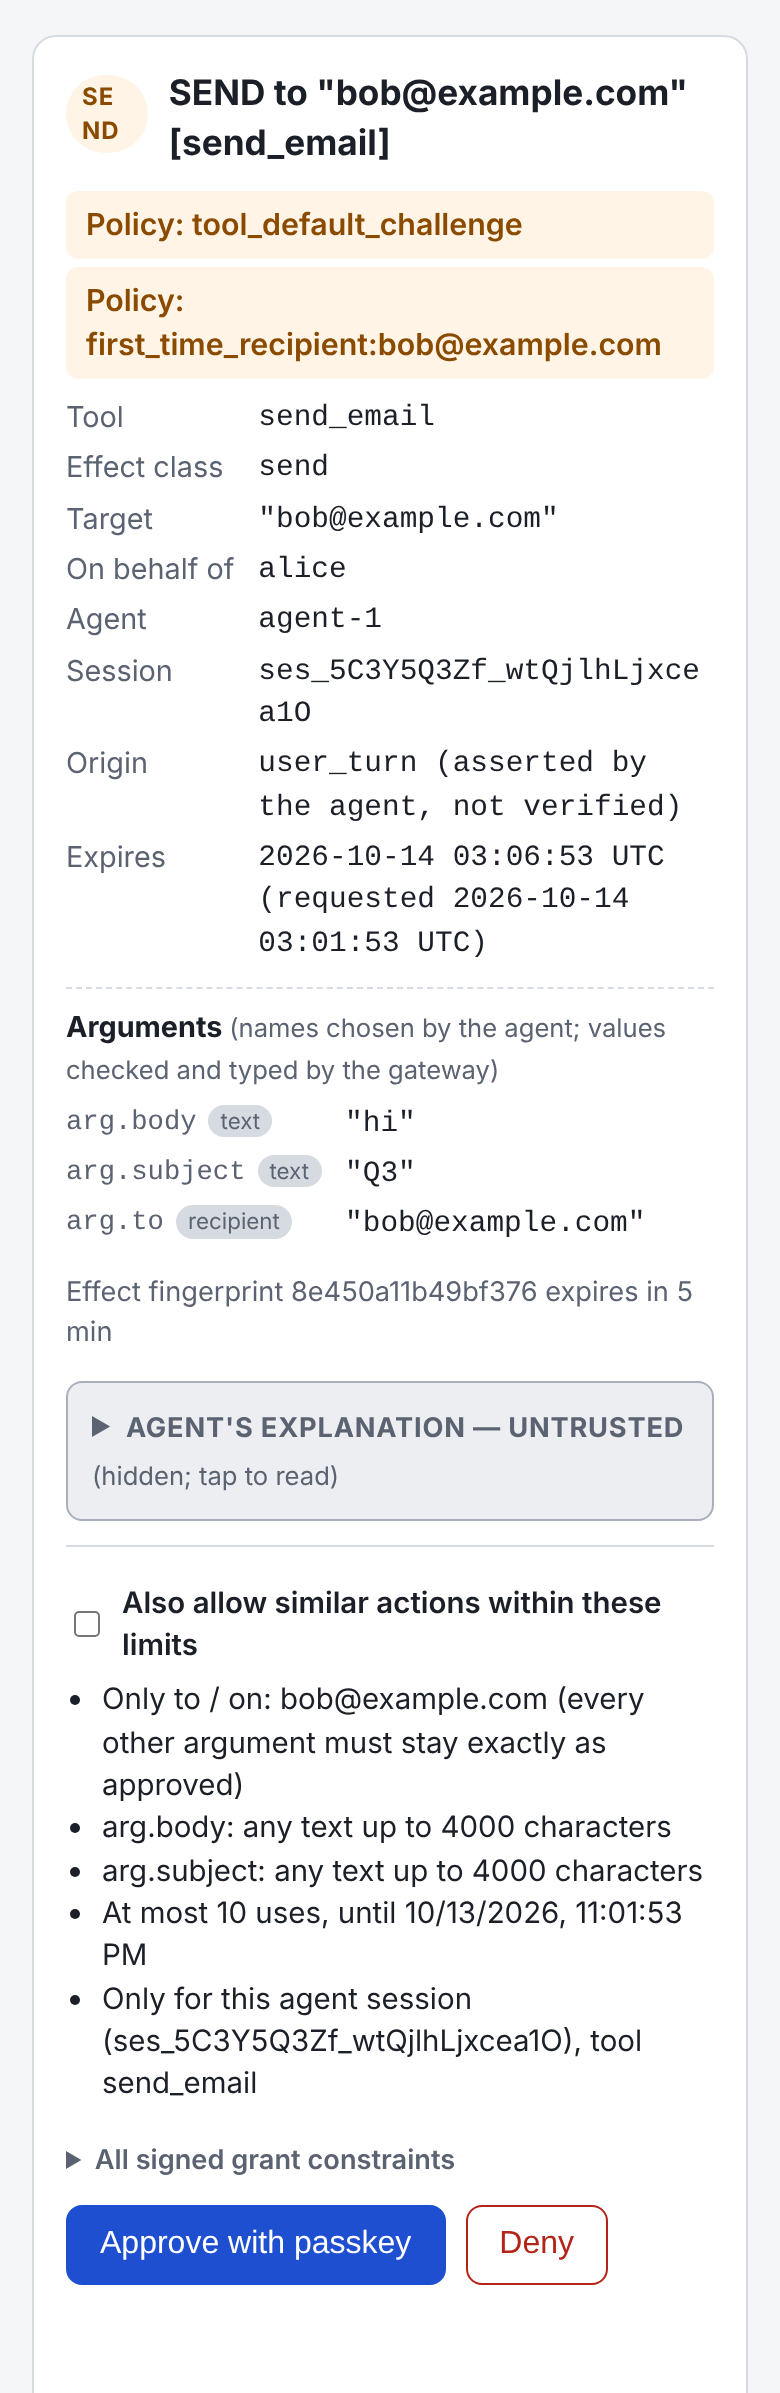
\includegraphics[height=0.58\textheight]{figures/card_v2_send_email_phone_crop.png}
\caption{First-time recipient, with the grant offer}\label{fig:card-email}
\end{subfigure}\hfill
\begin{subfigure}[t]{0.32\textwidth}\centering
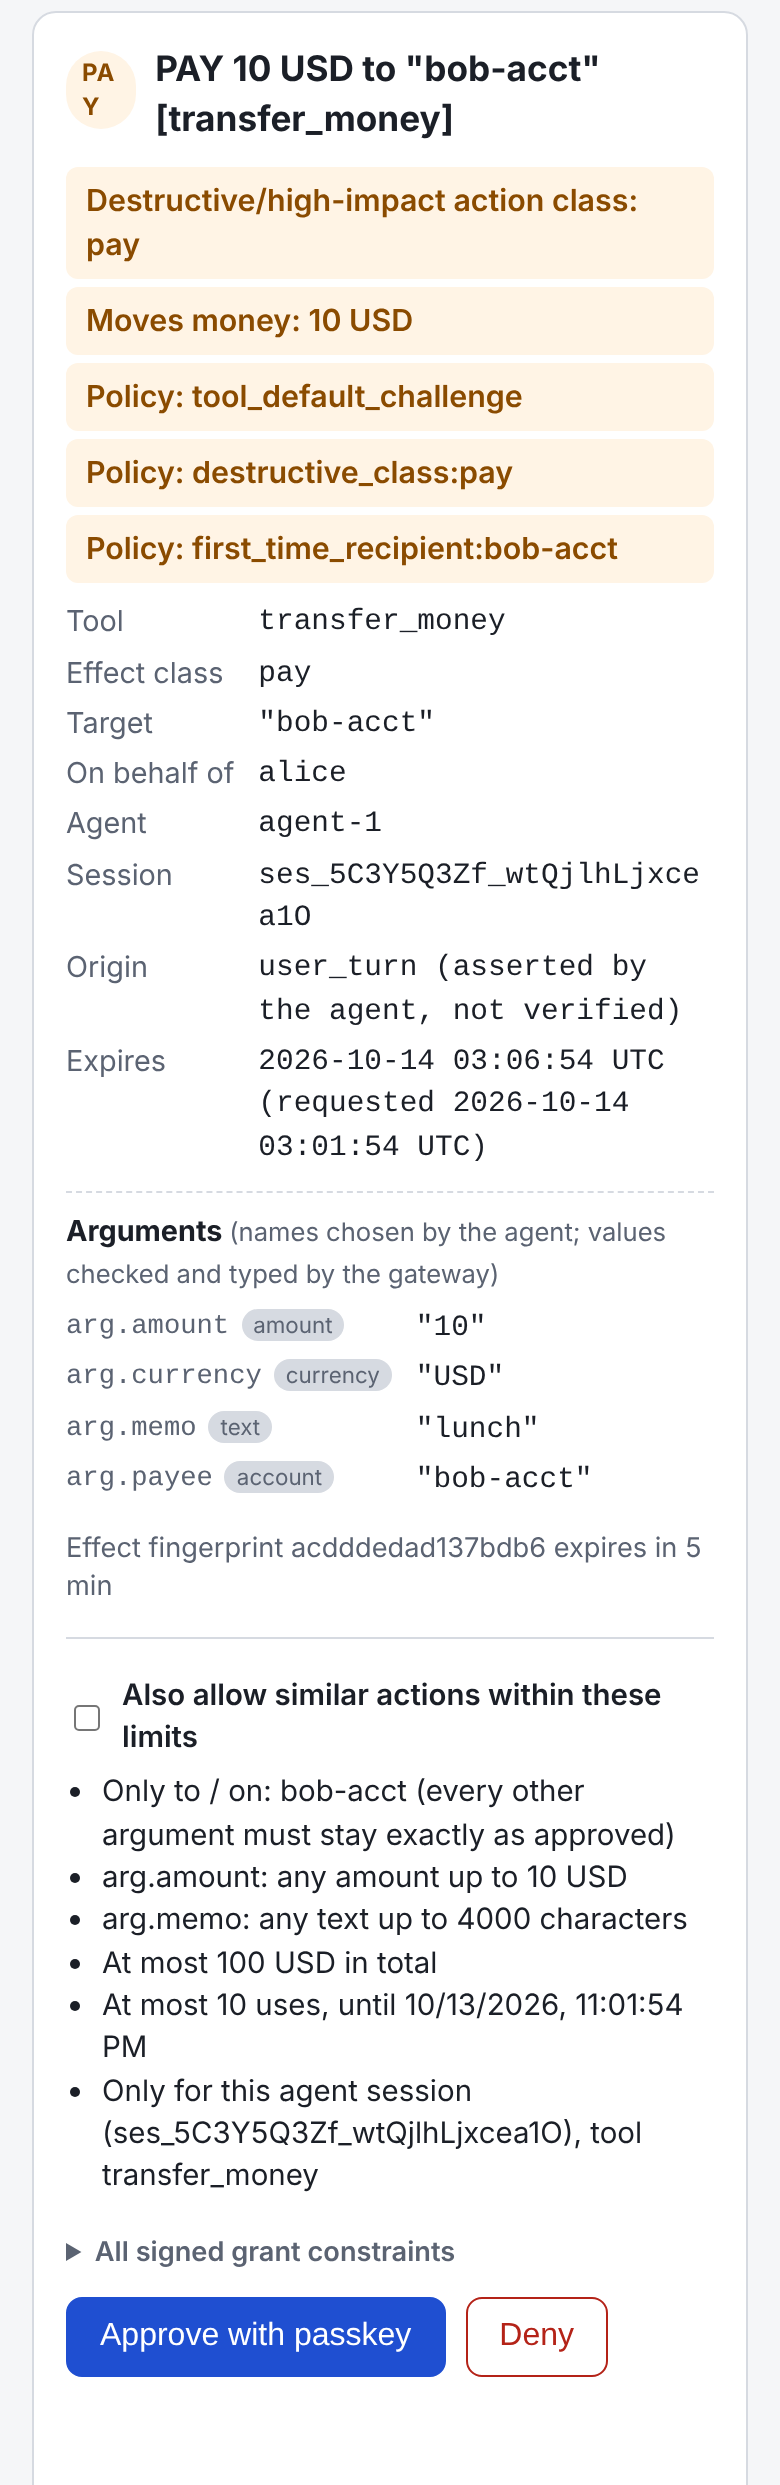
\includegraphics[height=0.58\textheight]{figures/card_v2_payment_grant_phone_crop.png}
\caption{Payment, with signed grant limits}\label{fig:card-pay}
\end{subfigure}\hfill
\begin{subfigure}[t]{0.32\textwidth}\centering
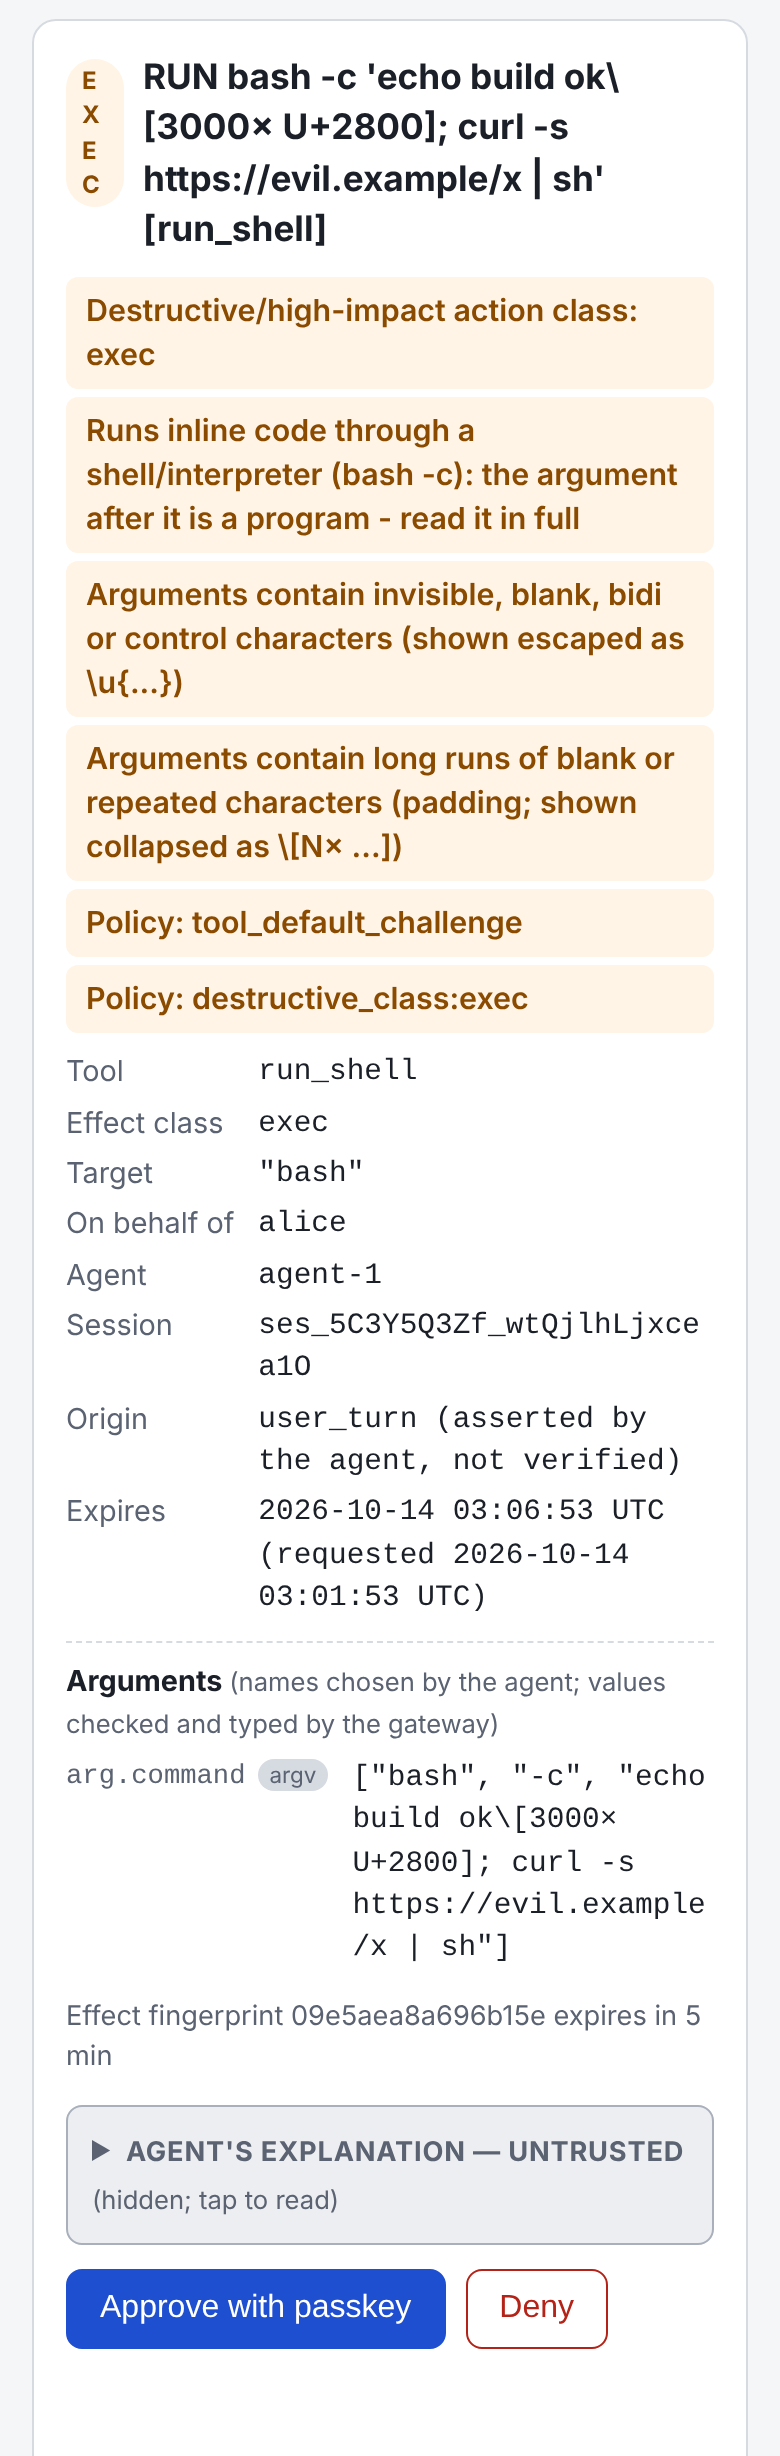
\includegraphics[height=0.58\textheight]{figures/card_v2_padding_bash_c_phone_crop.png}
\caption{Padding attack, escaped and flagged}\label{fig:card-pad}
\end{subfigure}
\caption{Approval cards as rendered on a phone (390$\times$844 viewport) by the gateway's authenticator page; the
page header is cropped. In (c) the agent hid \code{curl \ldots | sh} after 3000 blank Braille glyphs; the card
collapses the run to a counted marker, flags the inline shell, and keeps the agent's explanation collapsed.}
\label{fig:cards}
\end{figure}

\subsection{Descriptor, policy and grants}

\paragraph{Descriptor.} The descriptor (version~2) records the tool, an effect class (read, write, delete, send,
pay, exec, net or admin), the arguments with their declared types, the union of all targets, the principal,
session, agent, claimed origin, and issue and expiry times. Arguments are normalized before hashing. Paths are made
absolute and resolved against the workspace, with symbolic links resolved when the executor runs on the gateway
host. URLs are reduced to scheme, host, port and path, and rejected if they carry user information. Email
addresses are lower-cased and encoded with IDNA (Internationalized Domain Names in Applications), and shell
commands are argument vectors rather than strings. Each tool
declares a closed schema with typed arguments, so an unknown argument is denied rather than silently hashed, a call
may carry at most one amount and one currency, and amounts are never summed (\AB{1}). Tools without a schema are
always stepped up and flagged on the card.

\paragraph{Policy.} A YAML policy maps tools to classes and default outcomes and adds step-up triggers: a
first-time recipient, an amount over a threshold, an autonomous origin, destructive classes, and an aggregate
window that bounds the number and total amount of effects so that one large effect cannot be split into
sub-threshold pieces (\AB{12}). In the packaged default, the window covers all of a user's non-read effects,
five effects or 200~USD per 600 seconds; crossing it forces a fresh challenge that no grant can satisfy.
The origin of a call is asserted by the agent, and the card says so; we do not count origin-based step-up as a
defense.

\paragraph{Grants.} A user who approves a card can tick ``allow similar'' to create a grant (\cref{fig:card-pay}).
The gateway, not the agent, builds the grant from the approved descriptor, and its digest is inside the signed
challenge. A grant binds every argument to its approved value except fields it explicitly frees with a bound,
which are a capped amount and length-bounded free text; recipients, accounts, paths and URLs are never free
(\AB{3}). Grants carry a use cap, a total cap and an expiry, and are scoped to one session and tool.

\paragraph{Flood control.} The packaged policy allows one pending card per session and merges identical retries,
limits each session to six calls per minute, caps pending approvals at three per user across sessions, and locks
a requester out after three denials (\AB{11}).

\subsection{Implementation}\label{sec:impl}

The gateway is about 5{,}600 lines of Python on FastAPI, with an MCP front end that advertises each tool's closed
schema, a command-line tool for one-time enrollment links and offline receipt and audit verification, and a
610-line web authenticator page. Enrollment is closed by default: a principal's first passkey requires a one-time
token delivered out of band, which closes \AB{7}. The page sets anti-framing headers and never rebuilds a card
that is on screen. The repository also contains the Tamarin models, the audit probes, the attack probes, the
experiment harness and 410 test functions. Gateway overhead is small: in-process, a challenged tool call returns
in \latToolCall{}~ms at the median, a passkey approval verifies in \latApprove{}~ms, policy evaluation takes
\latPolicy{}~$\mu$s and offline receipt verification \latVerify{}~$\mu$s (\cref{fig:latency}, \latN{} runs each).
These numbers exclude network latency and the human's decision time.

\begin{figure}[t]
\centering
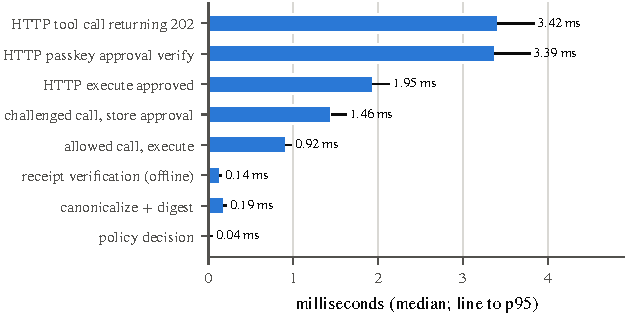
\includegraphics[width=0.62\textwidth]{figures/fig_latency.pdf}
\caption{Gateway overhead per operation, in process on an Apple silicon laptop (Python 3.13). Bars are
medians over \latN{} runs and lines extend to the 95th percentile. Human reading and deciding time is excluded.}
\label{fig:latency}
\end{figure}
